\section{Sparse Grids}
\label{sec:23sparseGrids}

\minitoc{67mm}{4}

\noindent
The idea of sparse grids is to use the
hierarchical splitting \eqref{eq:hierSplittingMV}
to keep only the most important hierarchical subspaces,
omitting the remaining ones.
There are three main ``flavors'' of sparse grids:
regular, dimensionally adaptive, and spatially adaptive.



\subsection{Regular Sparse Grids}
\label{sec:231regularSG}

\paragraph{Hierarchical contributions}

To assess the importance of a subspace, we consider again the
interpolant $\fgintp{\*l} \in \ns{\*l}$ of a function $\objfun\colon \clint{\*0, \*1} \to \real$.
According to the splitting \eqref{eq:hierSplittingMV}, the interpolant can
be written as
\begin{equation}
  \label{eq:interpHierFullGrid}
  \fgintp{\*l}
  = \sum_{\*l'=\*0}^\*l \sum_{\*i' \in \hiset{\*l'}}
  \surplus{\*l',\*i'} \basis{\*l',\*i'},\quad
  \falarge{\*i = \*0, \dotsc, \*2^\*l}{\fgintp{\*l}(\gp{\*l,\*i}) = \objfun(\gp{\*l,\*i})}.
\end{equation}
The coefficients $\surplus{\*l',\*i'}$ with respect to the hierarchical basis
$\basis{\*l',\*i'}$ are the \term{hierarchical surpluses.}
When using the hat function basis $\bspl{\*l,\*i}{1}$,
one can prove the following representation
for the corresponding surpluses \multicite{Bungartz04Sparse,Garcke13Sparse}:
\begin{equation}
  \label{eq:surplusIntegral}
  \surplus{\*l',\*i'}
  = (-1)^d 2^{-\normone{\*l'+\*1}}
  \int_\*0^\*1 \bspl{\*l',\*i'}{1}(\*x)\,
  \partialderiv[2d]{\partialdiff x_1^2 \dotsm \partialdiff x_d^2}{\objfun}(\*x)
  \diff{}\*x,
\end{equation}
if $\*l \ge \*1$ and
$\objfun$ is twice continuously differentiable in every dimension simultaneously,
i.e.,
$\partialderiv[2d]{\partialdiff x_1^2 \dotsm \partialdiff x_d^2}{\objfun}$
exists and is continuous.%
\footnote{%
  Again, the notation implies that the integration domain is
  the unit hyper-cube $\clint{\*0, \*1} = \clint{0, 1}^d$.%
}\multiplefootnoteseparator%
\footnote{%
  The statement is even valid for functions in the Sobolev space
  $H_\mathrm{mix}^2(\clint{\*0, \*1})$ with dominating mixed derivative,
  as its proof mainly relies on integration by parts
  \multicite{Bungartz04Sparse,Garcke13Sparse}.%
}
Consequently, the contribution of the summand of level $\*l$
can be estimated by
\begin{equation}
  \label{eq:componentEstimation}
  \normLtwoscaled{
    \sum_{\*i' \in \hiset{\*l'}}
    \surplus{\*l',\*i'} \bspl{\*l',\*i'}{1}
  }
  \le 3^{-d} \cdot 2^{-2 \normone{\*l}} \cdot
  \normLtwoscaled{
    \partialderiv[2d]{\partialdiff x_1^2 \dotsm \partialdiff x_d^2}{\objfun}
  }
\end{equation}
for the hat function surpluses $\surplus{\*l',\*i'}$
\multicite{Bungartz04Sparse,Garcke13Sparse}.

\paragraph{Definition of regular sparse grids}

Equation \eqref{eq:componentEstimation} motivates to omit those summands
from the sum \eqref{eq:interpHierFullGrid} whose level sum $\normone{\*l}$
exceeds a certain value $n \in \natz$,
as their contribution can be neglected compared to the summands
with coarser level sums.
More formally, the selection of the relevant subspaces can be formulated as a
continuous knapsack problem~\cite{Bungartz04Sparse},
assuming homogeneous boundary conditions.
\usenotation{zzzzs}
This motivates
\begin{equation}
  \label{eq:regularSG}
  \regsgspace{n}{d}
  \ceq \bigoplus_{\normone{\*l} \le n} \hs{\*l},\qquad
  \regsgset{n}{d}
  \ceq \bigdotcup_{\normone{\*l} \le n}
  \{\gp{\*l,\*i} \mid \*i \in \hiset{\*l}\}
\end{equation}
as the definitions for the \term{regular sparse grid space} and
\term{regular sparse grid} of level $n$, respectively.
The functions $\regsgintp{n}{d}$ contained in
$\regsgspace{n}{d}$ have the form
\begin{equation}
  \label{eq:regularSGInterpolant}
  \regsgintp{n}{d}
  = \sum_{\normone{\*l} \le n} \sum_{\*i \in \hiset{\*l}}
  \surplus{\*l,\*i} \basis{\*l,\*i}.
\end{equation}
To better distinguish the different grids,
we call the grids corresponding to the nodal spaces \term{full grids.}
We generalize the definition to arbitrary bases $\basis{\*l,\*i}$,
although sparse grids have been motivated using the hat function
basis $\bspl{\*l,\*i}{1}$
(the estimate \eqref{eq:componentEstimation} does not hold anymore
in the general case).
\Cref{fig:regularSG} shows the construction of a
regular sparse grid in two dimensions.

\begin{figure}
  \subcaptionbox{%
    Hierarchical splitting and subspace selection.
    The rectangles indicate the support of the
    bivariate hat basis functions.%
  }[85mm]{%
    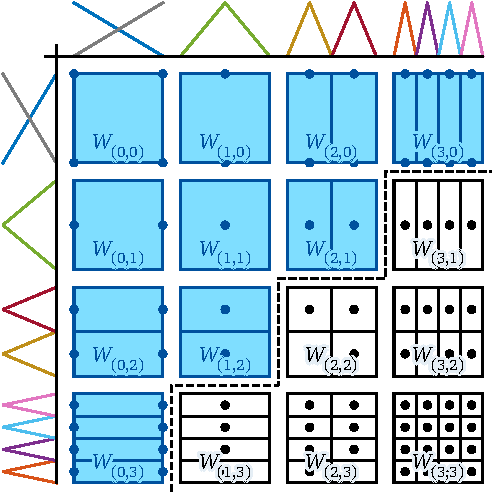
\includegraphics{sg_1}%
  }%
  \hfill%
  \begin{minipage}[b]{59mm}
    \subcaptionbox{%
      Full grid obtained by adding all subspaces of level $\*l \le n \cdot \*1$.%
    }[59mm]{%
      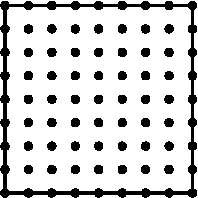
\includegraphics{sg_2}%
    }\\[4mm]%
    \subcaptionbox{%
      Regular sparse grid obtained by adding all subspaces
      whose level $\*l$ satisfies $\normone{\*l} \le n$
      \emph{\textcolor{mittelblau}{(blue)}.}%
    }[59mm]{%
      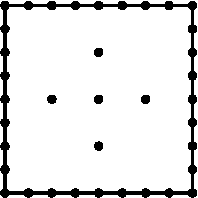
\includegraphics{sg_3}%
    }%
  \end{minipage}%
  \caption[%
    Regular two-dimensional sparse grid%
  ]{%
    Regular sparse grid of level $n = 3$ in two dimensions.%
  }%
  \label{fig:regularSG}%
\end{figure}

\paragraph{Grid size and interpolation error}

One can prove that for homogeneous boundary conditions
$\restrictfcn{\objfun}{\bndrydomain{\clint{\*0,\*1}}} \equiv 0$,
the number of required inner grid points
($\gp{\*l,\*i} \in \regsgset{n}{d}$ where $\*l \ge \*1$)
grows like $\landauO{\ms{n}^{-1} (\log_2 \ms{n}^{-1})^{d-1}}$
\multicite{Bungartz04Sparse,Garcke13Sparse}, which is much less than
the corresponding number $\landauO{(\ms{n}^{-1})^d}$ in the full grid case
(see \eqref{eq:dimensionFG}).
The $\Ltwo$ error of the sparse grid interpolant
$\regsgintp{n}{d} \in \regsgspace{n}{d}$ using hat functions
(still assuming homogeneous boundary conditions) decays like
\begin{equation}
  \normLtwo{\objfun - \regsgintp{n}{d}}
  = \landauO{\ms{n}^2 (\log_2 \ms{n}^{-1})^{d-1}},
\end{equation}
which is only slightly worse than the full grid error by the factor of
$(\log_2 \ms{n}^{-1})^{d-1}$
\multicite{Bungartz04Sparse,Garcke13Sparse}.



\subsection{Dimensionally Adaptive Sparse Grids}
\label{sec:232dimensionallyAdaptiveSG}

The idea of dimensional adaptivity is to spend more grid
points along specific dimensions depending on the objective function.
Different criteria for the choice of dimensions exist,
for example the maximal absolute value of the linear hierarchical surpluses.
To incorporate dimensional adaptivity into sparse grids,
one has to generalize the symmetric
choice of subspaces in the definition of regular sparse grids
to allow asymmetric preferences.
Generally, function spaces~$\sgspace$ and grid sets $\sgset$
of \term{dimensionally adaptive sparse grids} have the form
\begin{equation}
  \label{eq:dimensionallyAdaptiveSG}
  \sgspace
  = \bigoplus_{\*l \in \levelset} \hs{\*l},\qquad
  \sgset
  = \bigdotcup_{\*l \in \levelset} \{\gp{\*l,\*i} \mid \*i \in \hiset{\*l}\},
\end{equation}
where $\levelset$ is a \term{downward closed} set, i.e.,
a finite subset $\levelset \subset \natz^d$
for which $\fafa{\*l \in \levelset}{\*l' \le \*l}{\*l' \in \levelset}$.
Regular sparse grids are a special case by setting
$\levelset = \{\*l \in \natz^d \mid \normone{\*l} \le n\}$.

\paragraph{Combination technique}

The key advantage of dimensionally adaptive sparse grids over
spatially adaptive approaches is the
so-called \term{combination technique.}
For regular sparse grids, one can show that the sparse grid interpolant
$\regsgintp{n}{d}$ can be written as
\begin{equation}
  \label{eq:combiTechnique}
  \regsgintp{n}{d}
  = \sum_{q=0}^{d-1} (-1)^q \binom{d-1}{q} \sum_{\normone{\*l} = n-q}
  \sum_{\*i=\*0}^{\*2^\*l} \interpcoeff{\*l,\*i} \basis{\*l,\*i},
\end{equation}
where the $\interpcoeff{\*l,\*i} \in \real$ ($\*i = \*0, \dotsc, \*2^\*l$)
are the interpolation coefficients on the full grid
$\fgset{\*l}$ of level~$\*l$, i.e.,
$\fa{\*i' = \*0, \dotsc, \*2^\*l}{%
  \sum_{\*i=\*0}^{\*2^\*l} \interpcoeff{\*l,\*i} \basis{\*l,\*i}(\gp{\*l,\*i'})
  = \objfun(\gp{\*l,\*i'})%
}$ \multicite{Smolyak63Quadrature,Zenger91Sparse}.
For general dimensionally adaptive sparse grids, a similar formula exists
\cite{Nobile16Adaptive}.
The combination formula \eqref{eq:combiTechnique} splits the
sparse grid interpolant into a weighted sum of full grid interpolants
(see \cref{fig:combinationTechnique}).
In applications, each grid can be processed in parallel,
drastically speeding up computations like the solution of \pdes{}
\cite{Heene18Massively}.
In addition, existing code working on nodal bases does not have to be
rewritten in terms of implementing hierarchical functions,
which means that the combination technique allows sparse grids to be employed
in existing software in a minimally invasive way.

\begin{SCfigure}
  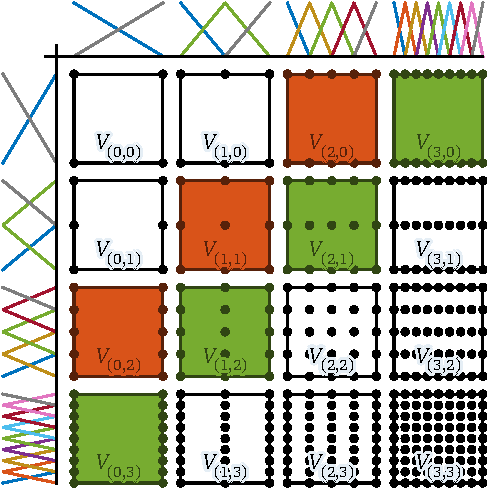
\includegraphics{sg_4}%
  \caption[%
    Sparse grid combination technique%
  ]{%
    The combination technique combines nodal subspaces in a weighted
    sum to form a regular sparse grid space of level $n = 3$ in two dimensions.
    The \textcolor{C1}{red subspaces} ($q = 1$ in \eqref{eq:combiTechnique})
    are subtracted from the sum of the
    \textcolor{C4}{green subspaces} ($q = 0$).%
  }%
  \label{fig:combinationTechnique}%
\end{SCfigure}



\subsection{Spatially Adaptive Sparse Grids}
\label{sec:233spatiallyAdaptiveSG}

Dimensional adaptivity does not suffice to resolve local features of the
objective function.
Especially in some applications, it is crucial for the
interpolant to be highly accurate in specific regions of the domain.
For instance in optimization, it is not necessary to have a small global
interpolation error.
Instead, high accuracy near the optima is important.

This can be achieved by \term{spatially adaptive sparse grids,}
on which this thesis focuses.
Generally, their function spaces $\sgspace$
and grid sets $\sgset$ have the form
\begin{equation}
  \label{eq:spatiallyAdaptiveSG}
  \sgspace
  = \spn\{\basis{\*l,\*i} \mid (\*l,\*i) \in \liset\},\qquad
  \sgset
  = \{\gp{\*l,\*i} \mid (\*l,\*i) \in \liset\},
\end{equation}
where $\liset$ is a finite set of level-index pairs $(\*l,\*i)$
with $\*l \in \natz^d$ and $\*i \in \hiset{\*l}$.
An example for a spatially adaptive sparse grid is shown in
\cref{fig:spatiallyAdaptiveSG}.

\begin{figure}
  \subcaptionbox{%
    Hierarchical splitting and grid point selection.
    The rectangles indicate again the support of the
    bivariate hat basis functions.%
  }[85mm]{%
    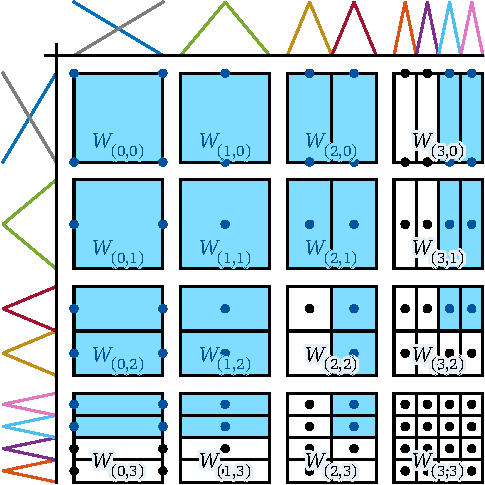
\includegraphics{sg_5}%
    \hspace*{1.411224mm}%
  }%
  \hfill%
  \subcaptionbox{%
    Resulting spatially adaptive sparse grid.%
  }[59mm]{%
    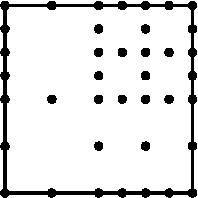
\includegraphics{sg_6}%
  }%
  \caption[%
    Construction of spatially adaptive sparse grids%
  ]{%
    Spatially adaptive sparse grid in two dimensions.
    More grid points were generated in the top right corner,
    which can help to resolve fine oscillations of the objective function.%
  }%
  \label{fig:spatiallyAdaptiveSG}%
\end{figure}

Algorithms for sparse grids often make specific assumptions about $\liset$.
If they are not met, then the algorithms do not produce the correct results.
For example when working with hat functions $\bspl{\*l,\*i}{1}$,
the grid should contain the hierarchical ancestors of every grid point.
Otherwise, the so-called unidirectional principle \cite{Balder94Adaptive},
which is used for instance to efficiently calculate
hierarchical surpluses, does not hold in general.
However, as we will see in \cref{chap:40algorithms},
the unidirectional principle cannot be applied
to B-splines of general degree, even if the hierarchical ancestors exist.
Hence, for most of our considerations, we will not restrict the
choice of $\liset$.
